\chapter{Recommender System}

Now that we learnt how to extract features from videos, those will be fed to a recommender system. In this chapter, we will explore various notable ways of building recommender systems, then dive into how we built ours. This section features various experiments showcasing the importance of various features and augmentation strategies.

\section{Problem setting}
\subsection{Lexicon}

A recommender system setting involves several entities.

\paragraph{The items} are the objects of interest of the application domain. For YouTube, it is videos, for Amazon they are products and for Spotify they are songs.

\paragraph{The platform} is the app. It can be Spotify, Facebook, YouTube, etc. The platform hosts items to recommend. They have their own set of goals, usually maximizing revenue.

\paragraph{Content creators}, on the aforementioned platforms, are the ones creating new items on the platform. Musicians for Spotify, user profiles for Facebook, shops for Amazon. Some platforms, such as Last.fm  (music recommendation) or MovieLens (movie recommendation) have no content creator. Instead, they have a catalog of items provided by the platform. The content creators have their own incentive for using that platform: they make revenue based on views, they sell items, they get exposure, etc. If the platform does not care enough about them, they might stop creating content and the platform loses its value.

\paragraph{Users} are the ones exploring the items and interacting with them. They are YouTube's viewers, Spotify's listeners, Amazon's shoppers, etc. Users find value in the platform for various reasons: it hosts items they value, it allows discovering new items they like, etc. If the platform does not have their interest at heart, they might leave, decreasing revenue to both the platform and content creators.

\paragraph{The recommender system} is a key element of the platform that has to solve a tripartite equation: maximizing its own business goals while maximizing the incentive for content creators to remain on this platform and to create more valuable content, and ensuring that users will get in contact with it. In other words, the recommender system has to find a mapping from content to users that is optimal for the three actors.

\subsection{At Hexaglobe}

Hexaglobe provides platforms for their clients. One major way a user interacts with content is by searching. In order to provide a good search engine, the platform has to extract features from behavioral patterns or from the content itself (description text, computer vision, etc); or to ask content creators for metadata about the item. Face recognition, for the client I am working for, provides metadata that is valuable to index items, and this is complemented by other tags.

However, in some cases, we want to be able to suggest the videos the user wants even before they search for it. This is typical on landing pages where we want to suggest videos the user will enjoy. This is known as a recommender system as it recommends content to a given user, sometimes based on its profile info and/or browsing history.

I have been tasked with giving a shot at writing a recommender system for my client.

\section{Recommender systems are hard to build}

Recommender systems are hard to build. They face many challenges. We all bought a toilet seat once because the current one broke and then Amazon wanted us to buy more toilet seats for months like we were on some weird toilet seat collection spree. We all got angry at Spotify for playing a song we hate, at YouTube for recommending for the billionth time that video we kept ignoring purposefully. We try to give a few explanations of the challenges.

\subsubsection{No clear ground truth}

The main reason is that there is no clear answer or goal to maximize or even evaluate. The complex interactions outlined above, between the platform's, content creators' and users' interest has usually been disregarded as they are too hard to express, quantify and too business dependent. Instead, the researcher community has seeked to develop business agnostic frameworks, the most common one being to model user preferences through ratings or an item's relevance to a user.

It's impossible, by design, to work out an unambiguously labeled dataset for a strict supervised task. The algorithms introduced later that look unambiguous and completely supervised, aiming at predicting a rating is not predicting what to display. Sure, that viewer seems to like romantic comedy, but if the system recommends romantic comedy ad nauseam, he will probably get bored and angry at that recommendation bubble. That's even worse if that user liked ONE romantic comedy and the recommendation engine interprets too strongly that spurious signal.

\cite{recpurpose} analyses several ways recommender systems can serve different purposes, both from the users' and the platform's point of of view. As user purposes, they exemplify: show alternatives, show accessories, help exploration, entertainment, etc. For platform's purpose: create more demand, increase business success, increase activity, increase discoverability of items, learn about customers, etc.

The algorithms presented here follow the trend and present recommendation as analogous to rating prediction, but this is a fairly severe assumption.

\subsubsection{Recommendation bubble}

Recommender systems might have the tendency to not balance enough exploitation of safe or known items and exploration of other items. This locks users in a fairly limited subset of items, and limits their ability to discover content, or even giving the false impression that there is no other content.

You just bought a shelf, and now Amazon wants you to buy every other shelves. You listen to rock music, you've never ever been recommended a single rap song, etc. Those are recommendation bubbles. You are getting recommended only items that are similar to things you already know and like, without any exploration or novelty. Sometimes, this is expected and a good thing: if you hate some type of music, it's okay not being exposed to it. Sometimes, you are missing out: you're not being recommended this great movie just because your past watch session inclines you more towards movies of lesser popularity matching a bit more the features you like. Finally, it can also be plain detrimental: being a flat earther whose recommendations include more flat earth fake news and not a single scientifically valid and informative video. Having political point of views that keeps you from being exposed to opinions opposed to yours, but gets you recommendations of more and more extreme content. \citep{filterbubble, filterbubblebook}

Recommendation bubbles must be at least considered when building a recommender system, and whether to fight against it or not by adding some randomness or exploration bias to the system.

\subsubsection{Bias towards previous system}

Training a recommender system on historical data will bias predictions towards the old one. The new system might learn to recommend a popular item only because the previous system was biased and made it popular. Inversely, the new system might learn to ignore some content only because that content was ignored by the previous iterations and reached zero popularity. There are mitigating strategies to debias the learning procedure to some extent \citep{youtuberec}.

\subsubsection{Cold start}

Finally, what should be done with a new user or item? A new user might not have enough implicit or explicit feedback or information for the system to gauge their interest. A new item has not been seen yet and it's hard to know who it can be appealing to or if it is ever going to be popular. This is known as the \emph{cold start} problem.

\subsubsection{Fairness}

\begin{figure}
    \centering
    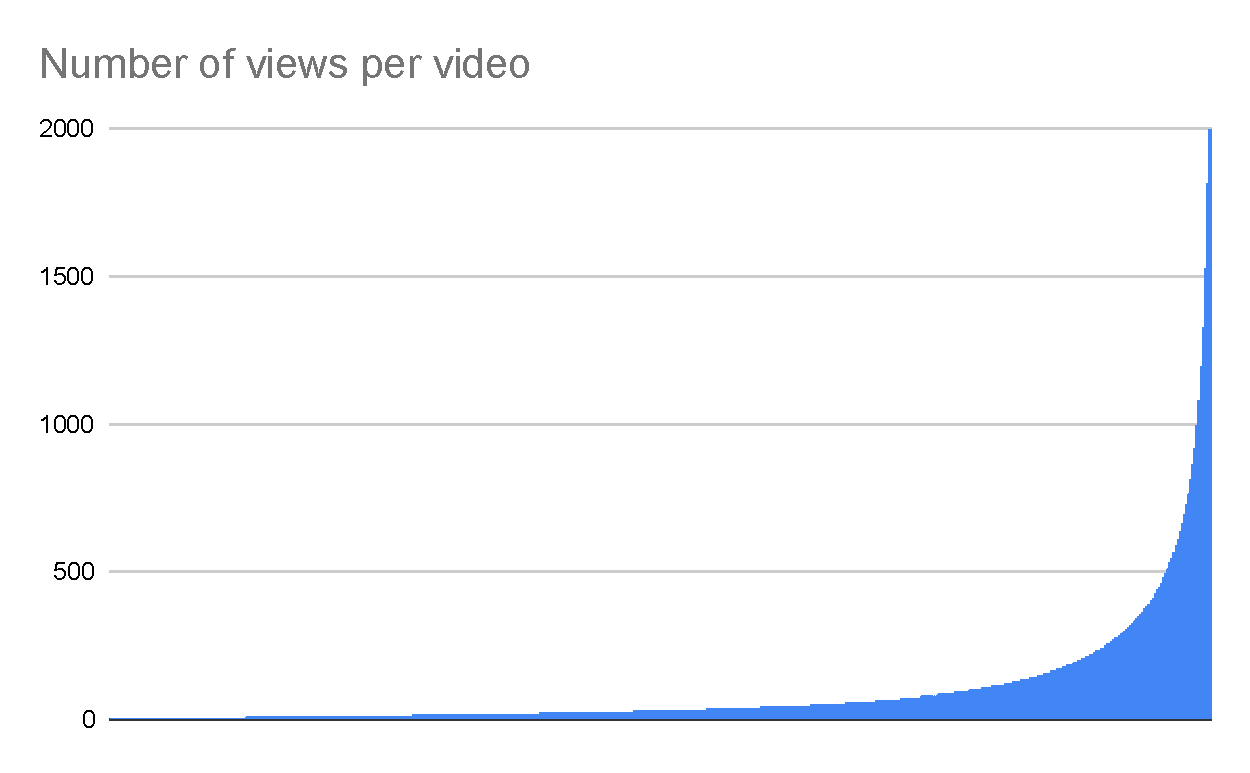
\includegraphics[width=\columnwidth]{70-files/long-tail.pdf}
    \caption{Long tail. A few popular items (the head) get a significant higher number of view than the majority (the tail). Exploiting only head items results in neglecting most items. The Y axis is clamped at 2k views but the highest video count is 8k.}
    \label{fig:long-tail}
\end{figure}

Related to the cold start problem is \emph{fairness}. Fairness might not matter for Netflix but might be of primal importance when the content is proposed by users, such as Amazon Marketplace or YouTube. Taking fairness into account is making sure that the system is not overly biased towards old and/or popular items, so that newcomers or smaller artists can still get recommended. Failing to account for fairness is making the system useless for the long tail items and narrowing the recommendations to top popular items. Users might benefit from more diversity and content creators get some benefit getting involved into the platform. \cite{popularitybias} inspects popularity bias, \cite{longtail} explores long tail items in music recommendation.

The long tail items are the ones - usually the majority - that get a much lower popularity than the top popular items. For some platforms, the value lies in exploiting the long tail items through personalization. It ensures that a valuable majority of items does not remain dormant. Figure \ref{fig:long-tail} shows the popularity distribution of my client's items. Failing to recommend long tail items would make it a bad platform for content creators and just a waste of hard drive space.

\section{Types of recommender systems}

\subsection{Definitions and notations}

Deciding what to recommend is difficult. To my knowledge, most recommender systems use ratings prediction as a proxy task. The datasets used contain user-to-items ratings from the platform history and the systems aim to predict how would users rate items they have not rated from the statistical knowledge extracted from previous ratings. They assume that the items with the best predicted ratings are the one to recommend.

Those algorithms assume that a given user $u_i \in \mathcal{U}$ emits explicit or implicit feedback ratings $r_{i,j}$ to content $c_j \in \mathcal{C}$. We have a sparse matrix of rating $r$ where row $r_{i,\cdot }$ represents ratings given by user $u_i$ and column $r_{\cdot,j}$ represents all ratings given to content $c_j$. From this, they want to predict $\hat{r}_{i,j}$, the rating for content $c_j$ that user $u_i$ would give.

\subsubsection{Collaborative filtering}

\begin{figure}
    \centering
    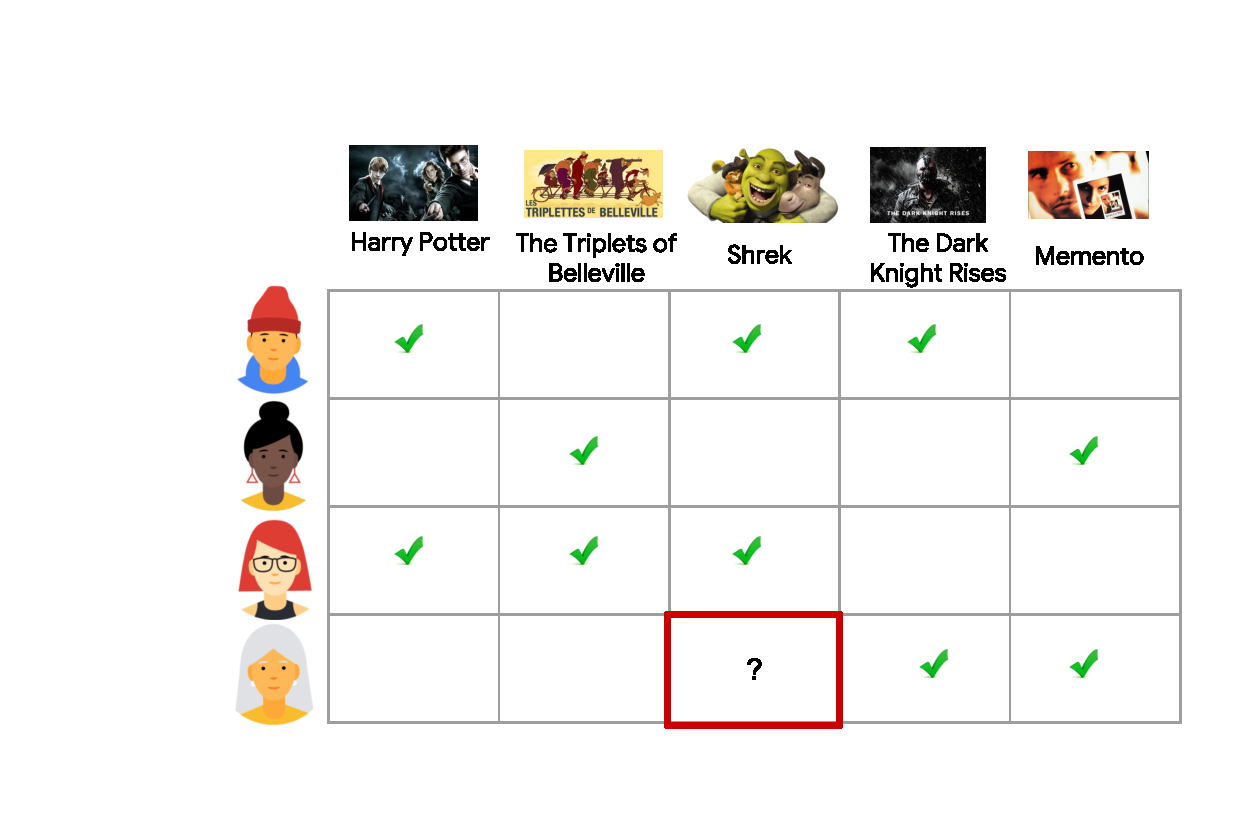
\includegraphics[scale=0.5]{70-files/collaborative-filtering.pdf}
    \caption{In collaborative filtering, we aim to guess the ratings one user would give to an item given the rating similar users gave. Would she like Shrek because she liked The Dark Knight like user 1, or dislike Shrek becaue she liked Memento like user 2?}
    \label{fig:collab-filtering}
\end{figure}

We can leverage information about a collection of user preferences. It is assumed that if a user $u_i$ shares opinion about some content with user $u_j$, then he should also share a similar opinion about another item that $u_i$ has not rated yet.

This method is often presented as "user who watched this video also watched", "users like you also liked". Figure \ref{fig:collab-filtering} displays a user rating matrix. The unknown value is predicted from the ratings of other users.

\subsubsection{Content-based filtering}

\begin{figure}
    \centering
    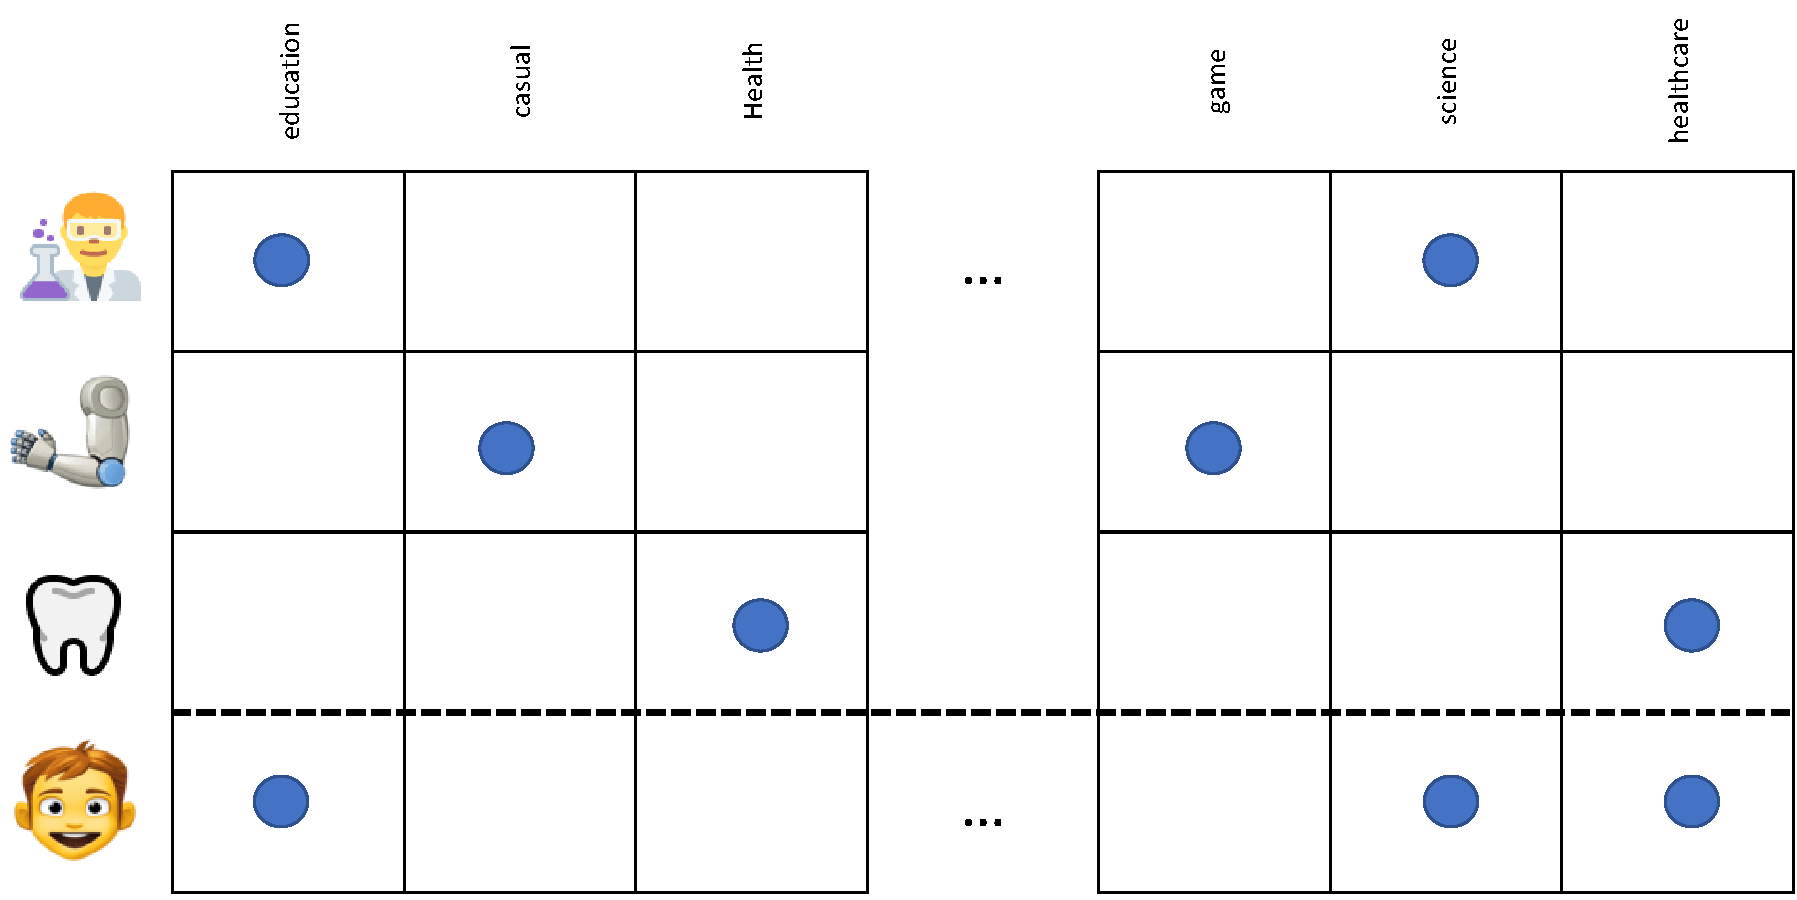
\includegraphics[scale=0.4]{70-files/content-based.pdf}
    \caption{This imaginary app store has 3 apps: a science app, a robot game, and a dentist appointment finder. Those apps and John's interests are annotated by a set of tags shown above the table. Based on John's past interests, the first item, the science app, seems to be a good recommendation: John's and this app's feature vector share the greater similarity.}
    \label{fig:content-based}
\end{figure}

In content-based filtering, a representation of items is extracted from some available features and metadata. An interest feature vector is extracted from a user's watch history and ratings, and the database of content is queried with it. A baseline algorithm uses \ac{TF-IDF} \cite{tfidf} for featurization and a dot-product for determining content relevance. Figure \ref{fig:content-based} shows a user's interests featurized in the same feature space as the items. Features could include keywords left in comments, main geographical region of users, and metadata might be categories and tags provided by the uploader. We recommend an item based on the user's similarity with candidate content. Contrarily to collaborative filtering, note that no other user is considered in making a decision. Platform presents content-based filtering such as "items matching your interests", or "similar to your recent history".

\section{Baseline algorithms}

\subsection{Deep learning is disappointing}

As in other areas, deep learning has been applied to recommendation for years, paper after paper. However \citet{dlinrec} ran a fair comparison between DL methods and carefully optimized baselines on common benchmark, and found out that DL methods were consistently outperformed. Those baseline work better and are orders of magnitude cheaper to run. For those reasons, the DL methods will not be detailed here. \citet{dlinrecseq} made similar findings for session-based recommender systems. It seems that deep learning models miss features-features interactions that make traditional methods work so well.

\subsection{Nearest neighbors}

\subsubsection{Base algorithm}

The $k$-Nearest-Neighbors algorithm allows to classify or regress to a value given a labeled training set. Let us lay a quick explanation of the method before applying it to our problem in the next paragraphs.

Let ${(x_0, y_0), ..., (x_N, y_N)}$ be a dataset of $N+1$ examples $x_i$ and their labels $y_i$. Classifying a query $q$ involves finding the $k$ most similar $x_i$ to $q$ under distance $d(\cdot, \cdot)$, and taking a majority vote of their class label $y_i$. For instance, if $k=1$,

$$kNN(q) = y_a; a = \arg \min_{i=0..N} d(x_i, q)$$

Here, we will use the cosine distance as the distance $d(\cdot, \cdot)$. In case of a regression task, the labels of the $k$ most similar items is averaged.


\subsubsection{kNN applied to recommendation}

To predict the ratings $\hat{r}_i,j$ that a user $u_i$ would give to a content $c_j$, \emph{UserkNN} takes the $k$ users most similar to $u_i$ and who have rated $c_i$. Their ratings value for item $c_j$ is averaged.


\emph{ItemkNN} takes the problem the other way around. We search for the $k$ items $c_k$ most similar to $c_j$ that had been rated by the active user $u_i$. The ratings that user gave to those similar items is averaged to predict $\hat{r}_{i,j}$.

There are multiple possible variations depending on how we decide to represent the users and items for the kNN:

\begin{itemize}
    \item The \emph{Collaborative filtering} uses the rating row $r_{i,\cdot}$ (column $r_{\cdot, j}$) to represent an user (item).
    \item The \emph{Content-Based Filtering} represents users and items by a set of features extracted from items metadata or user profile.
    \item An \emph{hybrid} method concatenates both metadata features and rating vector.
\end{itemize}

\subsection{Matrix Factorization}

\begin{figure}
    \centering
    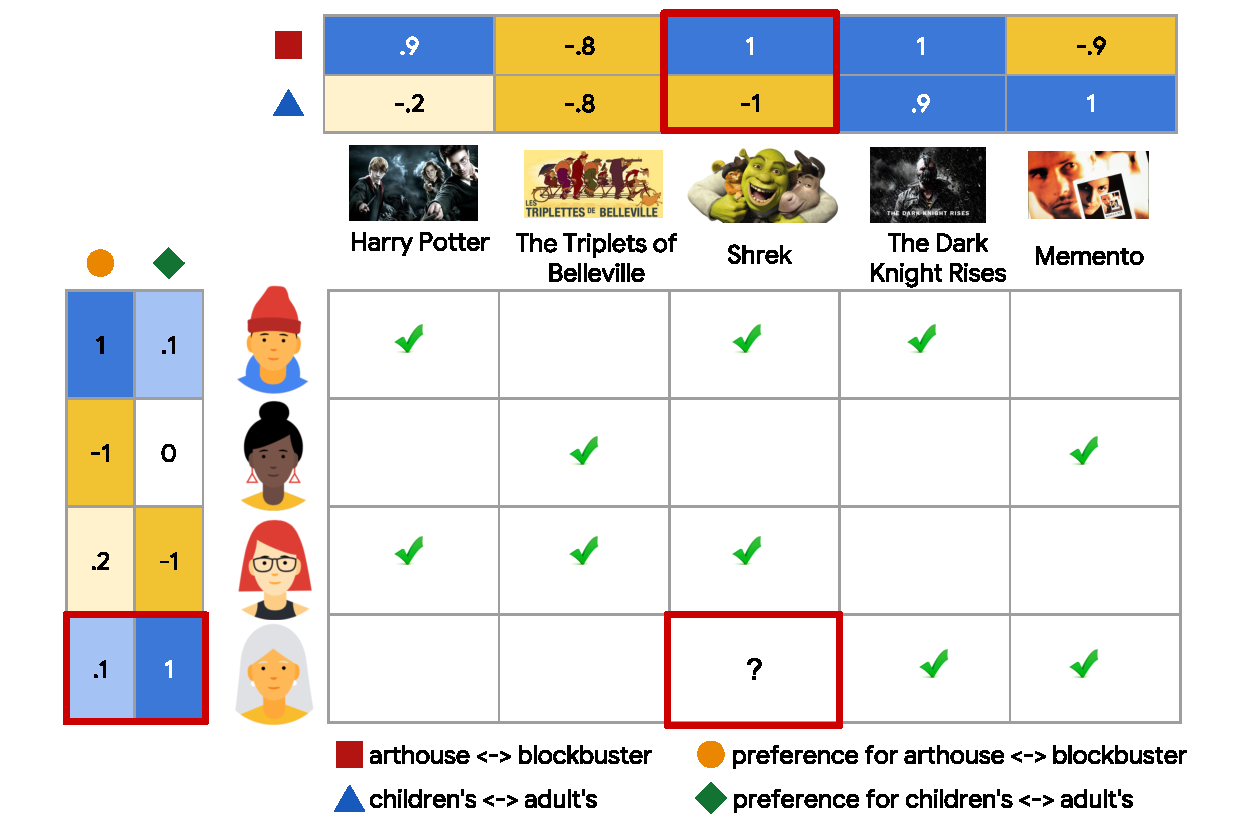
\includegraphics[scale=0.5]{70-files/matrix-factorization.pdf}
    \caption{The ratings matrix is decomposed as the inner product of user latent factors and movies latent factors, discovered during learning. They can be inspected to find semantically meaningful features. Image source: }
    \label{fig:matrixfactorization}
\end{figure}

\citet{funkmf} proposes a \emph{Matrix Factorization} approach that interprets the ratings matrix $r$ as the multiplication of a user matrix $A$ and a content matrix $B$ such that $r=AB^T$. Those matrices are of shape $|\mathcal{U}|\times k$ and $|\mathcal{C}| \times k$, where $k$ is a free parameter of the implementer's choice which represents the number of latent dimensions used to represent each user and content. We learn them when $r_{i,j}$ is known by minimizing the mean square error while regularizing both matrices

$$ \min_{A, B} (r_{i,j} - A_i \cdot B_j)^2 + \lambda ||A+B||^2$$

where $\lambda$ is the hyperparameter controlling the regularization strength. The unknown values can then be predicted $\hat{r}_{i,j} = A_i \cdot B_j$.

The greater $k$, the more latent factors can be learnt about users and items, the smaller the training error is but the overfitting risk increases. There are various ways to increase this model complexity and account for various biases or features.

Those embeddings can be analyzed to find semantically meaningful latent dimensions, like movie genre or target age group \citep{mflatents}. Illustrative examples are shown in figure \ref{fig:matrixfactorization}.

Pure MF methods need a full retrain at each new user, content or new interaction and suffer from a cold start problem : each user and content is treated independently. 

\subsection{SLIM: Sparse Linear Methods}

Instead of learning latent factors, one can learn how items recommend other items. \citet{slim} proposes to learn a $W \in \mathbb{R}^{|C|\times|C|}$ matrix representing the relation of items. $W$ is learnt by minimizing

\begin{equation}
\begin{split}
    & \min_W (r_{i,j} - r_i \cdot W_j)^2 + \lambda ||W||^2_2 + \beta ||W||_1 \\
    & \text{subject to} \\
    & W \geq 0, \text{diag}(W) = 0
\end{split}
\end{equation}

where $\beta$ and $\lambda$ are the hyperparameters regularizing, respectively, the $\ell_1$ aiming for a sparse $W$ and the $\ell_2$ norm preventing overfitting. The diagonal of $W$ is forced to zero so that items can't recommend themselves and fall into that trivial solution. Given that both $r$ and $W$ are very sparse, computing $\hat{r}=rW$ can be done very fast with sparse aware math libraries.

\subsection{$\text{EASE}^\text{R}$}

When the matrix $W$ of SLIM fits in memory, \citet{easer} proposes to remove the sparsity constraint and the positivity constraint. They devise a closed-form solution that allows for much faster learning. The results are on par or better than SLIM.

\section{\emph{\arr Project}: Hexaglobe's RecSys}

\subsection{Problem setting}

The client I am working for has 7M videos to index and recommend. They need recommendations in two places: on the homepage, and on a video page, as "continue watching" suggestions. The current homepage system is a country-wise top popular pick refreshed every hours mixed with some new uploads in order to fight the cold start problem. The "continue watching" suggestions are gathered from videos having similar search terms.

Despite many conversations, we could not fix an unambiguous single business objective to optimize. Do we want to optimize for retention? user fidelity? number of videos watched? watch percentage per video? They proposed subjective relevance evaluation with manual testing from the managers and client leader.

We could not agree on such a business centric metric, so we reverted back to a model metric, and judge our model based on its ability to recommend what the user watched next in the top-k recommendation. This is a Precision@k metric.

What should be further emphasized is that the baseline algorithms outlined above were very hardly applicable here. Indeed, the ratings are so scarce and unreliable on our client's platform that predicting ratings is not the option of choice here, despite its success. Instead, having profusion of users' watch history and metadata, it was easier to devise the problem as a sequence prediction setting.

\subsection{Contraints}

The system has some constraints to operate under in order to be useful in our production environment:

\subsubsection{Latency}
The system must return a recommendation response in under 30 ms

\subsubsection{Cold start for videos}
Around 15k videos are uploaded each day. Without a manual shuffling from our part or serendipity aware recommender algorithm, many of those videos would not get a single view, turning them into dead items. The system must not rely on collaborative features only for representing videos.

\subsubsection{Cold start for users}
Most users are not logged in when visiting the website. There is some cookie tracking done but users are not tracked between devices and many users browse our website in incognito mode. These constraints make it impractical to write a highly personalized engine. For these reasons, it has been decided to deploy the resulting engine on \emph{premium users} only first. Premium users should see the benefits of paying for their subscription as soon as possible or there is a risk of loosing them. This is a tight requirement that encouraged me considering seriously the user cold start problem as well.

\subsubsection{Fairness}
Even if it is secondary for the customer's business, dominated by big content creators, they want to encourage indie content creators. If it is not detrimental to recommendations, fairness is a desirable property to have.

\subsection{System design}

\subsubsection{Overview}

\begin{figure}
    \centering
    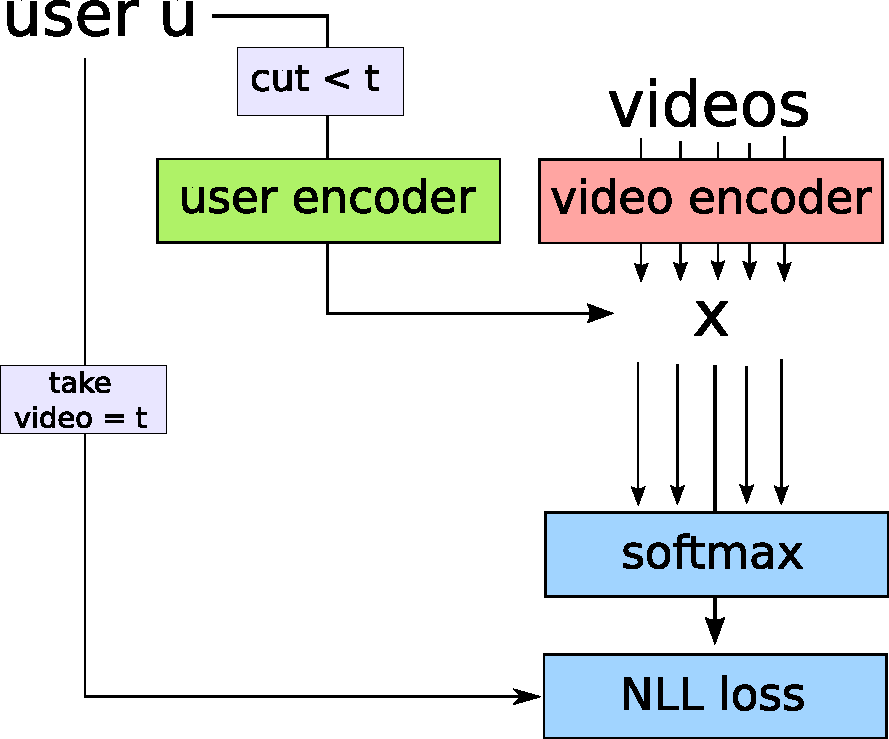
\includegraphics[scale=0.7]{70-files/xvrec-general.pdf}
    \caption{Overview of the model. We sample a user, randomly sample a video from the watch history, and cut the history at its watch timestamp $t$. The user is embedded by a user network while videos are encoded with a video network. The dot product of their embedding is computed and fed to a softmax + negative log likelihood loss, trained to predict the next video watched. The x denotes the dot product / matrix multiply operation.}
    \label{fig:xvrec-model}
\end{figure}

Back when I had to work on the recommender engine for Hexaglobe, the study of \citet{dlinrec} was not out yet and I chose to base my work on the Deep YouTube engine laid out by \citet{youtuberec}. This work proposes to learn a softmax classifier $f$ that predicts what a user $u$ will watch next. The user is represented by the profile and browsing history, while the videos are learnable embeddings in the last dense layer. Their function is designed to predict $y=f(u)$.

We propose avoiding the cold start problem by learning a user embedding function $f(u)$ and a video embedding function $g(v)$ for videos $v$. We predict the next video with 

\begin{equation}
    y=\text{softmax}(f(u) \cdot g(v)^T)
\end{equation}

Which is similar to the previous method but computes the video embeddings from a model instead of learning them as weights. This enables to use video metadata to generate embeddings, and possibly be more data efficient: $g$ has access to metadata to know which video are similar or not, instead of having to discover that from user behavior alone. Moreover, when a new video arrives on the platform, we can predict an embedding, instead of it being a dead item without user feedback, making it impossible to learn an embedding for it.

\subsubsection{User network}

The user network is a 2-layers MLP with 1024 hidden units and 64 output units. All categorical variables have an associated learnt embedding using pytorch's $\texttt{nn.Embedding}$ layer. When a categorical variable can take multiple values at the same time (like video tags), the embeddings of all tags are averaged, thanks to pytorchs's $\texttt{nn.EmbeddingBag}$. It encodes various features:

\begin{itemize}
    \item \textbf{Profile features}: country and gender. Categorical variables like those use learnt embedding before going into the MLP.
    \item \textbf{History features}: for the H previously seen, liked, favorited and disliked videos: their tags, their category, their main actors, their uploader's ID. The embeddings for all videos are concatenated. Sequences shorter than H are padded with zero embeddings. All the videos share the same embedding layers; there is no reason the tags from the last seen video must be encoded differently than the second to last. However, there is a reason to keep each video encoding separate, so that the network can estimate if the user's history is diversified or not, what was the previous seen videos so that it knows it can willingly decide to recommend it again or not, etc.
    \item \textbf{Request features}: for now, the category the user is browsing the website for. It was crucial making sure that the system would not recommend videos from another category as it displeases users. 
\end{itemize}

The dimension of the $\texttt{nn.Embedding}$ vectors is equal to $\min(512, 1.6n^{0.56})$ with $n$ being the number of possible values for this variable (following FastAI's rule of thumb).

\subsubsection{Video network}

The video network is similar to the user network. The input features are:

\begin{itemize}
    \item \textbf{Popularity features}: the popularity scores, summed over all categories.
    \item \textbf{Metadata features}: the category, the video tags, the main actors, the uploader's ID.
    \item \textbf{File features}: the video's encoding quality.
    \item \textbf{Optional: visual features}: convolutional features extracted for some images from the video.
\end{itemize}

The embedding layers for tags, actors, categories, and uploader ID are shared among both networks.

\subsection{Training strategies}

The data is sparse. There are a lot of different entities to embed, most of them being used rarely. In practice, this is a problem. The network could easily overfit and avoid learning a general recommendation function. Because they are rarely appearing, it may easily learn that tags 12, 68 and 98 identify video \#9786, and recognize user \#1234 from the history. The net would essentially learn nothing but a big table giving the ID of the next video given some user and timestamp and never form any semantic understanding.

In order to avoid such overfitting we propose to separately pretrain as much as the entities' embeddings as possible, and heavily regularize training.

\subsubsection{Pretraining tags and words embeddings with Word2Vec}


\paragraph{Word2Vec} was proposed by \citet{word2vec}. They learn words embeddings in a language-model fashion, exploiting words co-occurence. They either predict the probability of a center word $w_t$ at position $t$ its K left and right context words, or the opposite. $P(\texttt{center} | \texttt{context})$ is known as the Continuous Bag Of Words model while $P(\texttt{context}|\texttt{center})$ is known as the skip-gram model.

Once learned, those embedding display semantic properties, like similar words being clustered together or words showing linear relations. For instance, when training Word2Vec embeddings on general English corpus, we find that in this semantic space the vector from France to Paris is roughly the same as from Germany to Berlin.

Figure \ref{fig:word2vec} illustrates both CBOW and Skip-Gram models.

\begin{figure}
    \centering
    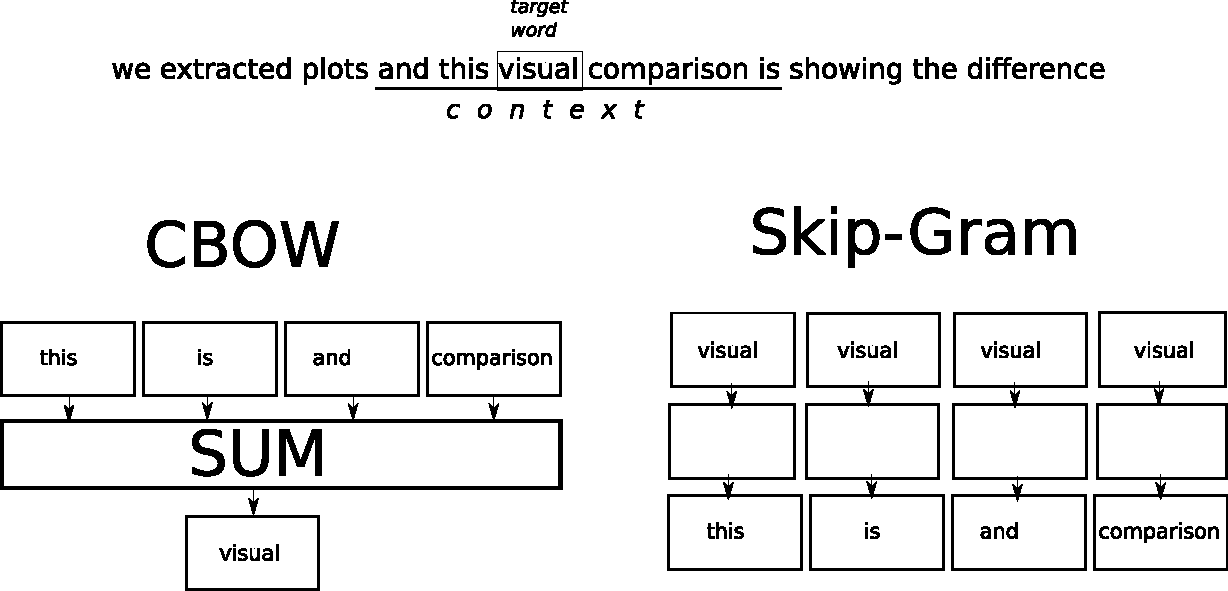
\includegraphics[width=\columnwidth]{70-files/word2vec.pdf}
    \caption{Illustrating word2vec training. A linear model trains word embeddings either by predicting the center word of a context window, or the context words of a context window from the center words.}
    \label{fig:word2vec}
\end{figure}

\paragraph{Tags} of a video, contrarily to words in a sentence, however, have no order. Deciding on a "center word" makes no sense, nor does "context window". We observe however that a user's watch history proposes a natural ordering. We thus considers all tags on a video to have the same position, and use the tags of previous and next videos as context. The target word is then a randomly picked word in the center video; tags from center and neighbouring videos are considered context as well. This already biases the embeddings towards recommendation. We use a context window of 5, that is, we use 2 videos before and after the center video as context.


We use the same strategy for words in the titles, also sampling context words, when applicable, from their multilingual translations. Stop words (pronouns, determiners, etc) that I am able to identify (French, English, Spanish) are removed.

Inspecting the embeddings with a technique such as UMAP \citep{umap} shows great insight about our tags. For instance, anime tags are effectively clustered together, such as various groups of tags for various genres, scene types, or famous actors. For this only, computing the Word2Vec embeddings has value. One could envision running a k-means algorithm on those embeddings to create invisible meta-tags that help even more with the indexing, merging different tags but with the same meaning.

Those embeddings are used, frozen, in the recommendation model.

\subsubsection{Regularization and data augmentation}

In order to both regularize the model and augment the data, dropout-based strategies are employed:

\begin{itemize}
    \item \textbf{DropTags}: There is a probability p to drop each tag in a video metadata.
    \item \textbf{RandLang}: Only one language is selected at random when there are multilingual data for the title
    \item \textbf{DropPop}: the popularity info is randomly dropped. This encourages fairness as well as the system learns not to recommend only videos with high popularity scores.
    \item \textbf{DropChannel}: Sometimes drops the channel ID. The system learns not to rely only on popular uploaders.
\end{itemize}


\subsection{What's next?}

Following the findings in \citet{dlinrec}, a simpler matrix factorization approach, not based on deep learning, might work better or just as well for a fraction of the compute. However, as mentioned earlier, those shallow approaches suffer from a generalization / cold start problem.

We could then learn a shallower system such as Matrix Factorization or build a collaborative filtering matrix for a user-knn or item-knn approach, disregarding (almost) inactive users and unpopular videos. 

For computing a score for a user or video (or both) not learned in the shallow model, a deep embedder net finds the closest known user / item, and the rating is taken from the corresponding entries in the shallow model.

\subsection{Experimenting with the model}

In order to gain insight into our dataset, choose our hyperparameters and refine the model, we run a collection of experiments. The model is trained with batch size 256 and Adam for 40k iterations. The learning rate warms up for 5\% of the training iterations then linearly decays. We train our model in a contrastive fashion: the batch contains 256 queries $x_{0...255}$ and their 256 associated next videos watched $y_{0...255}$. All queries and videos are embedded and the dot product is computed for all pairs so that the matrix $a_{ij}$ contains the dot product of the embedding of $x_i$ and $y_j$. A row-wise softmax is performed on $a$, and the cross entropy loss is computed so that row $i$ must predict label $i$. This strategy naturally samples according to the items' popularity, thus creating harder negative examples than uniformly sampling items. It also directly embeds the popularity bias of the items, forcing the system to rely on the features rather than learning which items are popular and finding them among long tail items. Top1 accuracy is used as a metric. We use a similar setting for testing.


\subsubsection{Candidate videos encoder}

We arbitrarily fix an history length of 2 with all user features as a starting point for running experiments. We add or ablate various features in the video encoder:

\begin{enumerate}
    \item A featureless experiment as a sanity check, making sure the accuracy is 1/256=0.39\%, which gives 0.395\%, passing the test.
    \item Only the category of the next requested item and candidate videos, giving 1.18\%. This is not surprising as there are only 3 main categories, which are notably unbalanced.
    \item Only the video encoding quality of the videos, giving 0.8\%. The video quality does not seem to explain much of the user behavior.
    \item Only the popularity scores, giving 5.86\%. This is quite surprising and would indicate that the dataset might not be enormously biased towards popular items. Or the popularity scores are computed in an unhelpful way.
    \item Only the uploader's ID, giving 20.25\%. It seems that this gives a lot of valuable information about the content, suitable for recommendation. A projection and visualization of the learnt uploader ID embeddings would help understand the semantic space they are organized into, and help get insight into the information extracted from the uploader ID.
    \item Only 3 tags per video, giving 9.33\%. Tags embeddings have 64 dimensions.
    \item Only 5 tags per video, giving 12.27\%. There are substantial gains adding more tags.
    \item Only 10 tags per video, giving 15.09\%. Adding more tags still helps.
    \item Only 15 tags per video, giving 19.37\%. Adding even more tags still helps.
    \item Only 20 tags per video, giving 20.80\%. This yields diminishing returns, 15 looks good for tests.
    \item Only 10 tags per videos, tags are pretrained, giving 17.92\%. This is a notable improvement from the random initialization. Does it help unfreezing the embeddings?
    \item Only 10 tags per videos, tags are pretrained and trainable, giving 19.22\%. Unfreezing tags embeddings help. Since we are challenging the performance with 15 tags, try with 15 pretrained and trainable tags.
    \item Only 15 tags per videos. Tags are pretrained and trainable, giving 22.74\%. The gains are still important.
    \item Uploader ID and 10 tags per videos. Tags are pretrained and trainable, giving 24.63\%. The uploader ID and tags do not bear totally redundant information.
    \item Uploader ID and 15 tags per videos. Tags are pretrained and trainable, giving 24.98\%. The uploader ID seem to bear enough information so that more tags yield diminishing returns.
    \item Uploader ID, 15 pretrained and trainable tags, category, quality, gives 25.45\%. This value serves as an upper bound when all info is available.
\end{enumerate}

We now have a pretty clear view of the importance of candidate video features. We settle to 15 pretrained and trainable tags, not using popularity scores (favoring unbiased information), with uploader ID, main category and quality.

\subsubsection{User encoder}

Now, we run feature experiments on the user encoder.

\begin{enumerate}
    \item We remove all features from users, giving 0.3905\%. Sanity check passes, without features, we get 1/256 chances of being right.
    \item Only profile geolocation features, gives 1.84\%. This is surprising as location correlates with language which can be inferred, to some extent, from tags. We know that language does not constitutes a major feature of our videos, but the accuracy gain still looks quite low.
    \item Only requested category gives 1.20\%. This matches the previous results with main category only in candidate videos.
    \item Only profile gender feature gives 0.6\%. Unsurprisingly, gender is a low indicator of user preference.
    \item Only 15 video tags from history gives 21.44\%. This jumps accuracy close to its maximum observed value.
    \item 15 video tags from history, video categories, request category, gives 22.77\%.
    \item Only Uploader ID from history gives 20.33\%.
    \item 15 Tags, category from history, uploader IDs from history, and request category gives 24.32\%.
    \item Enabling all user features, growing from 2 to 5 elements in history increases from 25.45\% to 25.59\%. This is not enough for the increased computation.
    \item Using all user features, only 15 tags in candidate video encoder but only viewed videos in history, gives 22.54\%. Only dislikes yields 3.51\%. Only likes 4.58\%. Views and like, 22.40\%. Views and dislikes, 22.37\%. All of them, 22.74\%. We see that, contrarily to intuition, likes and dislikes bears little information compared to views. Moreover, this information is not only redundant but maybe slightly misleading, suggesting not using likes and dislikes in the model.
    \item Using only views, categories, uploader ID, we reach 24.04\%.
    \item Using all data but gender (ie tags, categories, geolocation, uploader), with only past views from history, we reach 24.75\%. We consider that adding geolocation, even if it does not bring tremendous improvement, is very cheap and assume that it biases favorably the suggestions for a new user with localized 
    \item 25.05\% with views, likes and dislikes, confirming the improvement is marginal.
\end{enumerate}

We settle with a user encoder that uses all data but gender (ie tags, categories, geolocation, uploader), with only past views from history, reaching 24.75\%.

\subsubsection{Transforms}

We now evaluate our transforms.

\begin{enumerate}
    \item We activate DropTags with probability 0.25, effectively randomly dropping a quarter of the tags during training. It gives 24.78\%, making no difference. Raising to 0.5 probability yields 23.89\%, impairing the training. DropTags is better kept off.
    \item We activate DropChannel with probability 0.25 gives 24.63\%. Probability 0.5 gives 24.37\%.
\end{enumerate}

As it is sometimes the case with data augmentation, we experiment with less regularization and longer training schedule. We double the training time and reduce the weight decay from 0.1 to 0.01.

\begin{enumerate}
    \item Doubling the training iterations brings our baseline to 25.11\%. Adding DropTags with probability 0.25 yields 25.35\%.
    \item Reducing the weight decay brings our baseline to 24.91\%. Adding DropTags with probability 0.25 yields 24.05\%.
\end{enumerate}

\subsubsection{Further experiments}
We finally want to evaluate the contribution of face recognition to the recommender system. Adding the detected identities as features goes to 26.84\%, demonstrating a noticeable effect in recommending content. The identities embeddings could be pretrained with word2vec, in a similar fashion to tags embeddings, maybe yielding even greater improvements

\subsection{Discussion}

Starting from \cite{youtuberec} we designed our own recommender system, guided with experimental results. We found out that tags are by far the most important features to be used, followed by uploader ID as each uploader has its own type of content. We expected our model to overfit and devised some data augmentation techniques; the experiments showed that overfitting was not a problem but DropTags still managed to be helpful. We also showed that pretraining embedding with Word2Vec immensely helps, and the next steps to be be taken for maximum rewards are probably pretraining identity and channel embeddings as well, probably by predicting the associated tags distribution or their co-occurences in users' watch history. The practical use of this model now has to be tested in real world condition, and A/B testing is needed in order to compare it to the current recommender system to verify its superiority in actually understanding users' preferences.
